\documentclass{VUMIFPSbakalaurinis}
\usepackage{algorithmicx}
\usepackage{algorithm}
\usepackage{algpseudocode}
\usepackage{amsfonts}
\usepackage{amsmath}
\usepackage{bm}
\usepackage{caption}
\usepackage{color}
\usepackage{float}
\usepackage{graphicx}
\usepackage{listings}
\usepackage{subfig}
\usepackage{wrapfig}

% Titulinio aprašas
\university{Vilniaus universitetas}
\faculty{Matematikos ir informatikos fakultetas}
\institute{Informatikos institutas}  % Užkomentavus šią eilutę – institutas neįtraukiamas į titulinį
\department{Programų sistemų bakalauro studijų programa}
\papertype{Bakalauro baigiamasis darbas}
\title{Krepšinio taisyklių pažeidimo automatinis nustatymas}
\titleineng{Recognizing violations of basketball rules using computer vision}
\author{Lukas Cedronas}
% \secondauthor{Vardonis Pavardonis}   % Pridėti antrą autorių
\supervisor{partn. prof., dr. Vytautas Ašeris}
\reviewer{lekt. Donatas Kimutis}
\date{Vilnius – \the\year}

% Nustatymai
% \setmainfont{Palemonas}   % Pakeisti teksto šriftą į Palemonas (turi būti įdiegtas sistemoje)
\bibliography{bibliografija}

\begin{document}
\maketitle

%% Padėkų skyrius
% \sectionnonumnocontent{}
% \vspace{7cm}
% \begin{center}
%     Padėkos asmenims ir/ar organizacijoms
% \end{center}

\sectionnonumnocontent{Santrauka}
Glaustai aprašomas darbo turinys: pristatoma nagrinėta problema ir padarytos
išvados. Santraukos apimtis ne didesnė nei 0,5 puslapio. Santraukų gale
nurodomi darbo raktiniai žodžiai. 
% Nurodomi iki 5 svarbiausių temos raktinių žodžių (terminų).
% Vienas terminas gali susidėti iš kelių žodžių.
\raktiniaizodziai{raktinis žodis 1, raktinis žodis 2, raktinis žodis 3, raktinis žodis 4, raktinis žodis 5}   

\sectionnonumnocontent{Summary}
Santrauka anglų kalba. Santraukos apimtis ne didesnė nei 0,5 puslapio.
\keywords{keyword 1, keyword 2, keyword 3, keyword 4, keyword 5}

\tableofcontents

\sectionnonum{Įvadas}
Įvade nurodomas darbo tikslas ir uždaviniai, kuriais bus įgyvendinamas tikslas,
aprašomas temos aktualumas, apibrėžiamas tiriamasis objektas akcentuojant
neapibrėžtumą, kuris bus išspręstas darbe, aptariamos teorinės darbo prielaidos
bei metodika, apibūdinami su tema susiję literatūros ar kitokie šaltiniai,
temos analizės tvarka, darbo atlikimo aplinkybės, pateikiama žinių apie
naudojamus instrumentus (programas ir kt., jei darbe yra eksperimentinė dalis).
Darbo įvadas neturi būti dėstymo santrauka. Įvado apimtis 2 –– 4 puslapiai.


Vaizdo atpažinimas kompiuteriu - tai sparčiai besivystanti sritis. Egzistuoja daug algoritmų, kurių pagalba galima atpažinti objektus. Sportas. //@todo fix Sudetingesniems objektams dažnai yra naudojami giliuoju mokymu paremti metodai, šiame darbe išnagrinėti keli iš jų.  
//@todo Krepšinyje atpažinimas state of the art

\section{Naudoti įrankiai}

Kompiuterinės regos ir taisyklių pažeidimo atpažinimo algoritmams įgyvendinti buvo pasirinkta Python programavimo kalba. Python – interpretuojama, lengvai skaitoma kalba, puikiai tinkama įvairioms problemoms spręsti \cite{Python}. Dėl kalbos paprastumo ji dažnai naudojama kompiuterinės regos ir giliojo mokymo srityse, kadangi kalba leidžia susifokusuoti į abstrakcijas. Kadangi kalba yra plačiai naudojama, nesunku rasti daug pavyzdžių bei šaltinių. 

Objektų atpažinimui buvo pasirinkta OpenCV biblioteka \cite{opencv}. Tai – nemokama biblioteka, plačiai naudojama spręsti kompiuterinės regos uždavinius, kurios fokusas – įgalinti kurti aplikacijas leidžiančias efektyviai spręsti kompiuterinės regos problemas realiu laiku \cite{BradskiOpenCV}.

Python paketų, įgyvendinančių įvairius kompiuterinės regos algoritmus ir pagalbines funkcijas, siuntimui ir jų valdymui naudota Miniconda \cite{conda}. Ši biblioteka leidžia susikurti skirtingas aplinkas su tam tikrais reikalingais Python moduliais ir jas itin lengvai keisti priklausomai nuo norimo vykdyti kodo.

Vaizdo apdorojimui neuroniniais tinklais naudojama PyTorch biblioteka \cite{pytorch}, skirta lengvai valdyti neuroninių tinklų modelius bei juos integruoti į Python kodą. Taip pat PyTorch įgalina vaizdo apdorojimą naudojantis GPU. 

Vaizdo medžiaga rinkta filmuojant Xiaomi Redmi 8 Pro kamera.  

\section{Vaizdo medžiagos paruošimas}

Šio darbo metu sukurtai programinei įrangai paruošta vaizdo medžiaga, kurioje žaidėjas atlieka įvairius judesius su krepšinio kamuoliu. Siekiant supaprastinti vaizdo atpažinimo algoritmą, medžiagai keliami reikalavimai yra: aiškiai matomas žaidėjas, telpantis į kadrą ir užimantis nemažą dalį vaizdo. Vaizdo atpažinimui pagal spalvą algoritmui žaidėjas taip pat privalo dėvėti skirtingų spalvų pirštines, batus bei mušinėti atskiros spalvos kamuolį. Žaidėjas turi būti kiek galima labiau skirtis nuo fono, kad algoritmas veiktų kuo efektyviau, kadangi įvairių formų ir spalvų objektai fone pasunkina tikslų atpažinimą. Vaizdo medžiagoje žaidėjas mušinėja kamuolį ir atlieka įvairius judesius, dalis kurių pažeidžia taisykles, pavyzdžiui – pamušinėjęs kamuolį jį pasiima į rankas ir padaro keletą žingsnių. Programinė įranga turi atpažinti, jog tai – taisyklės pažeidimas. Vaizdo kokybė yra itin svarbi siekiant tikslių rezultatų, todėl buvo filmuojama kuo didesne raiška – Xiaomi Redmi Note 8 Pro kameros maksimali raiška yra 4K, 30 kadrų per sekundę. 

\section{Vaizdo atpažinimo metodai}

Šiame darbe apibrėžtiems algoritmams, atpažįstantiems krepšinio taisyklių pažeidimus, reikalinga tam tikra pradinė informacija apie žaidėjo kūno dalis ar objektus (rankas, pėdas, kamuolį ir pan.). Ši informacija yra gaunama vaizdo įrašo kadrus apdorojant kompiuterinės regos metodais. 
Nagrinėjamus metodus galima sugrupuoti į tris grupes: 

\begin{itemize}
	\item Metodai, kurių pagalba remiantis kadre iš anksto žinomi spalvomis galima išskirti dominančius regionus (pvz. segmentavimas) bei metodai, papildomai apdorojantys gautus rezultatus (pvz. atliekant morfologines operacijas ar randant regionus apimančius kontūrus).
	\item Metodai, kuriais naudojantis atpažinimą vykdyti galima nepriklausomai nuo spalvų, pavyzdžiui, kamuolio atpažinimo algoritmas paremtas Hough transformacijomis, taip pat - judesio atpažinimas remiantis fono pašalinimu ir skirtumų tarp kadrų atradimu.
	\item Metodai paremti neuroniniais tinklais - žmogaus skeleto atpažinimas naudojantis OpenPose bei Lightweight modeliais. 
\end{itemize}

Skyriaus pabaigoje visi šie metodai palyginami praktiškai, sukuriant minimalų žingsnių skaičiavimo algoritmą, įgyvendintą minėtais metodais, išryškinant jų privalumus bei trūkumus. 

\subsection{Spalvinis atpažinimas}
Vienas iš būdų išskirti ir atpažinti objektus yra tada, kai žinome jų spalvą iš anksto. Šiam procesui egzistuoja daug metodologijų, pavyzdžiui, grupavimas, slenksčio nustatymas bei erdvės domenu paremti metodai, tokie kaip regionų auginimas, skaidymas ir sujungimas, grafiniai pjaustymai ar panašiai \cite{segmentation_trends}. Vienas iš slenksčio nustatymo ar grupavimo privalumų yra tas, kad be iš anksto žinamų ir suklasifikuotų spalvų rėžių atpažinimas nereikalauja daugiau a priori žinių apie paveikslėlį ar jame egzistuojančius objektus ir yra paprastai įgyvendinami \cite{segmentation_trends}. Spalvinio atpažinimo metodai, tarp jų ir slenksčio nustatymas, gali būti panaudojami tokioms problemoms spręsti, kaip žmogaus veido atpažinimas \cite{WANG20011983}. Pagal spalvų reikšmes galime išskirti regionus, juos reprezentuojant vienetukų ir nuliukų matricomis, ir su jomis atlikti įvairias logines operacijas tam, kad būtų galima palengvinti tolimesnį atpažinimą, pvz., pašalinant triukšmą. 

Tačiau tai, jog siekiant atpažinti ranką ar kamuolį būtina iš anksto žinoti, kokios spalvos bus tie objektai, yra vienas iš praktinių trūkumų: darosi sudėtinga išskirti atskiras kūno dalis naudojantis informacija apie odos spalvą, kadangi tikėtina, kad ne tik žaidėjo rankos, kojos bei veidas bus tos pačios spalvos, bet galimai sutaps ir su kitų žaidėjų. Taip pat dažnai sunku iš anksto žinoti, kokios spalvos apskritai reikia ieškoti, kadangi skirtingi žmonės gali turėti skirtingą odos spalvą ar ji gali keistis priklausomai nuo apšvietimo \cite{KAKUMANU20071106}. 

Dėl šių limitacijų siekiant ištirti spalvinių metodų efektyvumą ir pritaikomumą krepšinio žaidėjas turėtų iš anksto dėvėti tam tikros spalvos pirštines, batus bei valdyti ryškios spalvos kamuolį, tačiau realiame pasaulyje žaidėjus priversti nešioti skirtingų spalvų batus, pirštines būtų itin nepraktiška. Todėl šiame darbe taip pat bus nagrinėjami dar keli kompiuterinės regos atpažinimo būdai, nepriklausantys nuo spalvų. 

\subsubsection{Segmentavimas}
Segmentavimą kompiuterinėje regoje galima suprasti kaip radimą grupės panašių pikselių. Kai paveikslėliai segmentuojami pagal spalvą, panašumą galima išmatuoti pagal reikšmių skirtumą remiantis RGB arba HSV spalvų erdvėmis. Naudojantis vienu iš segmentavimo būdų - spalvos slenksčio (arba rėžių) nustatymu – OpenCV įgalina ganėtinai paprastai išskirti dominantį regioną, kadangi užtenka apsibrėžti tam tikrą intervalą spalvų paveikslėlyje, reprezentuotame trimate matrica, ir nufiltruoti matricos reikšmes nepatenkančias į duotąjį intervalą. 

RGB modelyje spalvą koduoja trimis reikšmėmis, nusakančiomis raudonumą, žalsvumą ir mėlynumą. Tačiau naudoti jį spalvinio atpažinimo metoduose yra sudėtinga - keičiantis apšvietimui nenuspėjamai gali pasikeisti spalvos RGB reikšmė. Egzistuoja algoritmai, gebantys atskirti apšvietimo pokyčius RGB modelyje \cite{1220504}, tačiau HSV modelis leidžia informacija apie atspalvį, ryškumą ir šviesumą saugoti kaip atskiras reikšmes. Šis modelis puikiai tinka spalvų atpažinimui, kadangi H (atspalvio) reikšmė mažai kinta paveikslėliuose atsiradus šešėliams \cite{1039893} ar miglotumui \cite{7457892}. Atspalvis dažniausiai išlieka tas pats nepriklausomai nuo pašalinių efektų, todėl lengva nusistatyti reikšmių intervalą. Konvertavimas iš RGB ir HSV yra pakankamai trivialus, OpenCV jis yra įgyvendintas cvtColor() funkcija. 

Turint intervalą užtenka nufiltruoti visus pikselius, kurių reikšmė nepatenka į duotą intervalą. Tiems, kurie patenka, loginėje matricoje priskiriamas 1, o tiems, kurie ne - 0. Rezultate gauname išskirtą regioną kur žinome, kad tai - tam tikras dominantis objektas, su sąlyga, kad jis vienintelis kadre buvo tos spalvos, pagal kurią vyko filtravimas. 
\begin{figure}[H]
	\centering
	\subfloat[\centering Vaizdas prieš segmentavimo pagal pirštinės spalvą]{{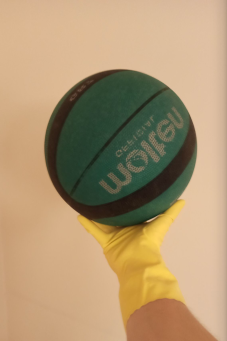
\includegraphics[width=5cm]{img/hand_before_segmentation} }}
	\qquad
	\subfloat[\centering Vaizdas po segmentavimo pagal pirštinės spalvą]{{
\includegraphics[width=5cm]{img/hand_after_segmentation} }}
	\caption{Segmentavimo pavyzdys}
	\label{fig:example}
\end{figure}

\subsubsubsection{Dominančių objektų spalvų rėžiai}
Atliekant bandymus pastebėta, jog net ir naudojantis HSV spalvų erdve, dominančių objektų spalvų rėžiai itin skiriasi priklausomai nuo apšvietimo.
Tikrieji HSV spalvos Jie skirdavosi net ir tarp skirtingų vaizdo įrašų. Šiame darbe naudojamų spalvų rėžiai //@todo add spalvos .

\subsubsection{Morfologinės transformacijos}
Atlikus segmentavimą pagal spalvą, rezultate dažnai lieka triukšmo ar bereikalingų artifaktų, kurie gali affectinti tolimesnį apdorojimą. @todo fix

Tokiais atvejais apsivalyti nuo triukšmo gan dažnai naudojamos slenkstinės (\textit{angl.} threshold) operacijos \cite[112]{SzeliskiCompVision}. Apsibrėžus tam tikrą filtrą, su juo galima atlikti operacijas ant matricų. Šiame darbe naudotos operacijos yra erozija ir plėstis. Erozija naudojama tada, norima sumažinti turimų atskirų regionų paveikslėlyje plotus, nuardant kraštus. Jei objektai yra pakankamai maži, o erozijos operacija - stipri (?), tuomet taip pašalinamas triukšmas. Formaliai erozija buvo aprašyta 1980 metais K. Y. Yoo \cite{4767941} kaip morfologinė operacija, sukombinuojanti dvi aibes naudojant vektorių atimtį aibių elementams. Matematiškai tai galima aprašyti tokia formule: 

\begin{equation}\label{eq:erozija}
	A \ominus B = \bigcap_ {b \in B } (A)_{-b} .
\end{equation}

\ref{eq:erozija} lygtyje A žymi dominantį paveikslėlį, išreikštą matrica, o B - filtrą arba kitaip - struktūrinį elementą, su kuriuo A matricoje pakartotinai atliekamos sankirtos.  

Erozijai priešinga operacija yra plėstis \cite{4767941}. Ši operacija leidžia padidinti išskirtų regionų plotą. Plėstis naudinga tuomet, kai po erozijos operacijos objektai praranda per daug ploto. Plėstį galima užrašyti šitaip:

\begin{equation}\label{eq:plestis}
	A \oplus B = \bigcup_ {b \in B } (A)_{b} .
\end{equation}

Atliekant bandymus pastebėta, jog siekiant geriausių rezultatų šalinant triukšmą, plėstį reikėtų vykdyti po erozijos, priešingu atveju triukšmas gali nebūti panaikintas. 

OpenCV įgyvendina funkcijas erode ir dilate, kurios priema paveikslėlio matricą ir struktūrinį elementą. Taip pat egzistuoja funkcija morphologyEx(), kuri, priklausomai nuo paduodamų parametrų keičia savo veikimą: su MORPH\_OPEN atliekama plėstis po erozijos, su MORPH\_CLOSE - atvirkščiai. 

\subsubsection{Kamuolio kontūrų radimas}

Siekiant iš paveikslikų išgauti daugiau kontekstualios informacijos, pavyzdžiui, ar kamuolys yra rankose, išsiskirti tarpusavy nesusikertančius regionus neužtenka. Tam, kad gauti šią informacijos dalį, reikia rasti, kada rankos ir kamuolio regionai susikerta, t.y. jų matricų sankirta yra netuščia. Tam reikia žinoti, kokią erdvę apima kamuolys - šios informacijos trūksta po segmentavimo pagal spalvą, jei kamuolys yra uždengtas, pavyzdžiui, rankos. 

Vienas iš būdų šią problemą išspręsti - pabandyti atspėti, kokią sritį užima kamuolys randant jo kontūrus. Skritulių kontūrams rasti 1991 metais E. Welzl pasiūlė algoritmą, rekursiškai apskaičiuojantį tam tikrai taškų aibei mažiausią ją apimantį apskritimą \cite{Welzl91smallestenclosing}. Šis algoritmas - tiesinio kompleksiškumo, jį įgyvendina OpenCV funkcija minEnclosingCircle().       

\begin{figure}[H]
	\centering
	\subfloat[\centering Kamuolio kontūrai prieš mažiausio aibę apimančio apskritimo radimo algoritmą]{{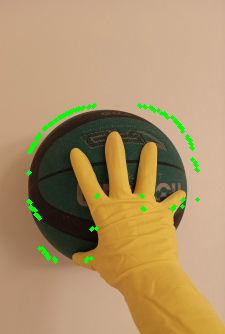
\includegraphics[width=5cm]{img/ball_contours_before} }}
	\qquad
	\subfloat[\centering Kamuolio kontūrai po mažiausio aibę apimančio apskritimo radimo algoritmo]{{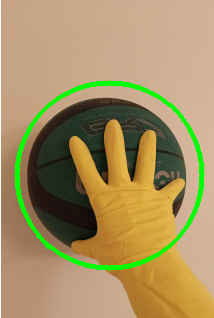
\includegraphics[width=5cm]{img/ball_contours_after} }}
	\caption{Kontūrų radimo algoritmo pavyzdys}
	\label{fig:example}
\end{figure}

\subsection{Atpažinimas remiantis skirtumais}
\subsubsection{Fono pašalinimas}
Fono pašalinimas yra vienas iš esminių metodų kompiuterinėje regoje, naudojamas išskirti dominančius vaizdus ir pašalinti nereikalingus statiškus objektus iš fono. Pavyzdžiui, jei yra filmuojama lauke, fone besimatantys medžiai gali trukdyti tolimesniam atpažinimui, tad žinant, jog mus domina tik žaidėjas, pašalinius objektus galima pabandyti pašalinti. Vienas iš būdų yra iš anksto turėti fono paveiksliuką ir apdorojant kitus kadrus jį išimti, bet tai dažnai nepasiteisina dėl to, kad fonas gali kisti – gali atsirasti šešėlių, pasikeisti apšvietimas, gali būti įvairaus pašalinio judėjimo, pavyzdžiui – linguojantys medžiai, vaikštantys sirgaliai ir pan. 2002 m.  P. KaewTraKulPong pasiūlė algoritmą, išsprendžiantį šią problemą \cite{KaewTraKulPong2002}. Algoritmas kiekvieną pikselį sumodeliuoja į Gauso skirstinį pagal tai, kiek pikselio spalva keičiasi bėgant laikui. Kuo mažiau pikseliai keičiasi, tuo didesnė tikimybė, kad jie priklauso fonui. Naudojantis šiuo atradimu galima sėkmingai atsikratyti fono, taip išskiriant mus dominantį vaizdą. Šis metodas ypač tinkamas atpažinti judėjimui – vietoje stovintis žaidėjas bus priskirtas fonui, tačiau jam judant, lengvai galima išskirti jo siluetą.  

\begin{figure}[H]
    \centering
    \subfloat[\centering Vaizdas prieš fono pašalinimą.]{{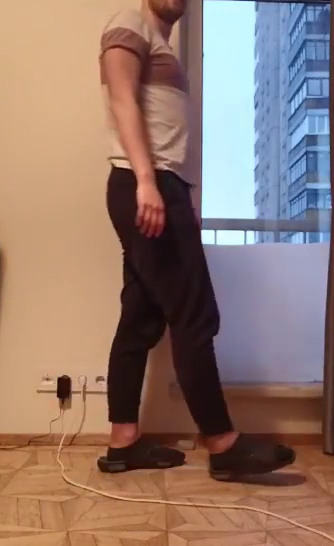
\includegraphics[width=5cm]{img/background-substraction-before} }}
    \qquad
    \subfloat[\centering Vaizdas po fono pašalinimo.]{{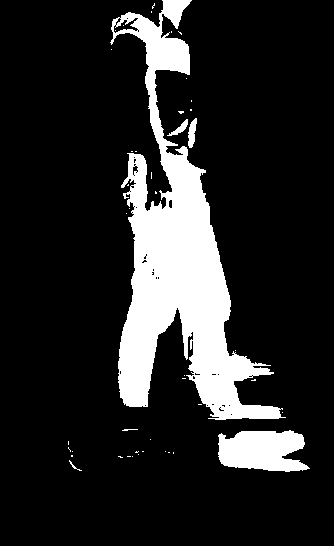
\includegraphics[width=5cm]{img/background-substraction} }}
    \caption{Fono pašalinimas naudojantis Gauso skirstiniu paremtu fono segmentavimo algoritmu.}
    \label{fig:example}
\end{figure}


Paveikslėlyje matome, jog algoritmas atpažino žmogaus siluetą. Šiame pavyzdyje ranka priskirta fonui dėl to, jog spalva sutampa su sienos spalva, tačiau kitos kūno dalys išskiriamos iš fono.

\subsubsection{Judesio atpažinimas}\label{section:movement}

Žaidėjui vaikštant, kai kurios kūno dalys juda greičiau, nei kitos. Kūnas išlieka santykinai statiškas palyginus su kojomis. Žingsniavimo mechanika yra tokia, kad atliekant žingsnį, viena koja lieka vienoje vietoje, kol kita yra perstatoma iš vienos pozicijos į kitą. Tam, kad pagauti tą kojos judesį, galima paprasčiausiai iš antro kadro atimti pirmą. Padalijus kadrą į dvi dalis – viršutinę ir apatinę – ir darant prielaidą, jog apatinėje dalyje matysis tik kojų judesiai, galima teigti, kad jei atėmus antrą kadrą iš pirmo yra skirtumas, buvo atliktas žingsnis. Koją pastačius ant žemės, tam tikrą laiką skirtumai sumažėja iki nustatytos ribos – pasinaudojus visa šia informacija galima apskaičiuoti, kiek žingsnių buvo atlikta. 

\begin{figure}[H]
    \centering
    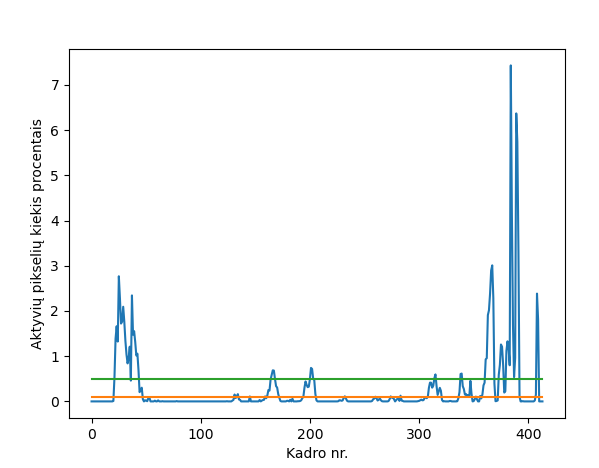
\includegraphics[scale=0.8]{img/steps}
    \caption{Aktyvių pikselių kiekis kiekviename kadre, indikuojantis žmogaus judėjimą. }
    \label{img:steps}
\end{figure}

\ref{img:steps} paveikslėlyje matyti, kiek buvo aktyvių pikselių kiekvieną kadrą panaudojus fono pašalinimą bei kadrų skirtumo algoritmus. Ši informacija rodo judėjimo kiekį tam tikrame kadro regione. Žalia linija žymi minimalų judėjimo kiekį, kuris gali atsirasti dėl triukšmo ir pašalinio judėjimo. Viršijus šią liniją galima teigti, jog žaidėjas šiuo metu juda. Oranžinė linija žymi ribą, iki kurios galima sakyti, jog jokio judesio nėra, t.y. žaidėjas pastatė koją ir ruošiasi atlikti kitą žingsnį. 

\subsection{Žmogaus kūno dalių atpažinimas neuroniniais tinklais}

Šiuolaikinėje kompiuterinės regos srityje daug naudos galima gauti pasinaudojus neuroninių tinklų pagalba. Neuroniniai tinklai naudojami sprendžiant įvairias problemas, šiam darbui aktualiausia yra objektų atpažinimo problema. Turint tam tikrą kadrą, taisyklių pažeidimo algoritmui būtina, kad būtų atskirtos rankos, kojos ir kamuolys. Žmogaus kūno dalių klasifikavimas yra sudėtinga problema, kadangi dauguma algoritmų yra priklausomi nuo surinktų duomenų. Kompleksija tampa akivaizdi sprendžiant sporto problemas, kadangi labai dažnai žaidėjai daro įvairiausius judesius, apsirengę įvairiausiais rūbais ir pan., kas apsunkina žaidėjo kūno dalių atpažinimą \cite{Andriluka_2014_CVPR}. Tam reikalinga turtinga ir didelė duomenų aibė, dėl ko neuroninio tinklo apmokymo laikas išauga. 

Bene visi šiuolaikiniai metodai remiasi tuo pačiu principu: apmokinamas neuroninių tinklų modelis, jiems paruošiant teigiamus ir neigiamus pavyzdžius (pvz., siekiant sukurti kojų atpažinimo algoritmą, paveiksliukai, kuriuose yra koja pažymimi kaip teigiami, tie, kuriuose kojos nėra tampa neigiamais). Mokinimo procesas gali trukti daug laiko – kartais net savaites, todėl daug paprasčiau yra pasinaudoti jau sukurtu modeliu. Vienas iš modelių, pavadinimu OpenPose, buvo pasiūlytas 2018 metais \cite{cao2019openpose}. Modelio architektūra paremta konvoliuciniais neuroniniais tinklais. Modelis suskirstytas į dvi šakas. Viena jų priskiria tikimybes, kad tam tikras regionas yra tam tikra kūno dalis, kita – asociacijas tarp skirtingų kūno dalių. Atpažinimas vyksta keliais etapais, siekiant gauti kuo tikslesnius rezultatus. 

Šiame darbe kuriamas vaizdo atpažinimo algoritmas kiekvieną kadrą pateikia OpenPose modeliui, o rezultate gaunamos skirtingomis spalvomis sužymėtos kūno dalys. Taisyklių pažeidimo atpažinimo algoritmui aktualios yra rankų ir pėdų sritis. 

\begin{figure}[H]
    \centering
    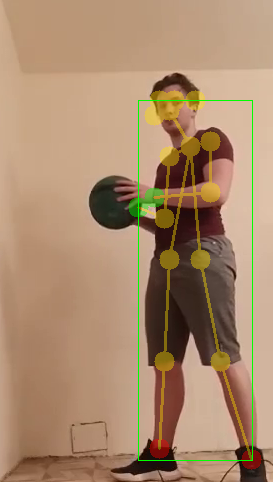
\includegraphics[scale=0.8]{img/body-parts-better}
    \caption{OpenPose algoritmo pagalba atpažintos kūno dalys.}
    \label{img:mlp}
\end{figure}

Vienas iš algoritmo trūkūmų yra tai, kad be optimizavimo su kiekvienu kadru gauti rezultatą užtrunka iki 0.5 sekundės. Galimas optimizavimo būdas yra sumažinti kadro dydį prieš pateikiant jį į neuroninį tinklą, tačiau tokiu atveju rezultatų tikslumas yra atvirkščiai proporcingas kadro dimensijom. 

2018 m. buvo pasiūlytas OpenPose modelio patobulinimas, įgalinantis žmogaus kūno atpažinimą beveik realiu laiku \cite{osokin2018realtime}. Lightweight optimizuoja OpenPose modelio architektūrą sumažinant sluoksnių skaičių, ryškiai pagerinant atpažinimo greitį nežymiai prarandant tikslumą. 

Atliekant bandymus su vaizdo medžiaga pastebėta, jog Lightweight modelis žaidėjo pozą atpažįsta ne tik greičiau, bet ir tiksliau. Eksperimentui buvo sukurti penki vaizdo įrašai, kuriuose žmogus atlieka tam tikrus veiksmus. Tikslumas buvo apskaičiuotas už teisingą kūno dalies atpažinimą kiekviename kadre pridedant 1 tašką, už neteisingą atpažinimą atimant 1, o gautą rezultatą padalinant iš kūno dalių skaičiaus, kurį atpažįsta modelis.

\begin{table}[H]\footnotesize
	\centering
	\caption{OpenPose ir Lightweight modelių palyginimas}
	{\begin{tabular}{|c|c|c|} \hline
			\textbf{Modelis} & \textbf{Vidutinė trukmė apdoroti vieną kadrą (ms)} & \textbf{Vidutinis rezultatų tikslumas (\%)} \\
			\hline
			OpenPose  & 581    & 62       \\
			\hline
			Lightweight  & 163    & 91       \\
			\hline
	\end{tabular}}
	\label{tab:openposevslightweight}
\end{table}

Dalį Lightweight modelio tikslumo pranašumo galėjo lemti OpenPose parametrų ir paduodamo kadro dimensijų neatitikimas, o spartumo - tai, jog duomenų apskaičiavimas OpenPose tinklu buvo įgyvendintas su OpenCV dnn moduliu, kuris bandymų metu nebuvo sukonfigūruotas naudoti GPU akceleravimą. Kadangi po optimizacijos Lightweight modelis tenkino tikslumo ir greičio lūkesčius, toliau nuspręsta naudoti jį. 

\subsubsection{Atpažinimo neuroniniais tinklais optimizavimas}

Atliekant bandymus pastebėta, jog atpažinimą Lightweight modeliu galima optimizuoti. Viena iš optimizacijų, kuri buvo atlikta, tai skaičiavimo perkėlimas ant GPU. Tam galima panaudoti CUDA - NVIDIA sukurtą API parareliems skaičiavimams \cite{cuda}. OpenCV puslapyje rašoma, jog su CUDA paveikslėlių apdorojimas gali pagreitėti iki 30 kartų \cite{opencv-cuda}. Be GPU akceleracijos Lightweight tinklas vieną kadrą užtrukdavo apdoroti iki 680 ms. 

Pastebėta, jog apdorojimo greičiui įtakos turi ir kadro dimensijos. Jei į neuroninį tinklą paduodamo kadro plotis yra didesnis, nei jo aukštis, apdorojimo greitis pakyla iki 5 kartų. Tačiau tai buvo mitiguota atnaujinus OpenCV versiją iš 4.0.1 į 4.5.1 - po šio atnaujinimo, apdorojimo greičiai tapo nebepriklausomi nuo santykio tarp paveikslėlio aukščio ir pločio. 

Dar viena išbandyta optimizacija - neuroninio tinklo pradinio sluoksnio įvesties dydžio sumažinimas. Dvigubai sumažinus įvesties kanalų skaičių iš 256 į 128 rezultatų tikslumas pasikeitė sąlyginai nedaug. Žiūrint į vaizdo įrašą, plika akimi galima pamatyti, jog atpažintas skeletas yra labiau "klibantis", t.y. kiekvienos kūno dalies koordinatės nežymiai skiriasi, kai įvesties dydis yra mažesnis, tačiau pačios kūno dalys dažnai lieka atpažintos teisingai. Siekiant tikslesnių rezultatų, siūloma pasilikti prie 256 kanalų skaičio, tačiau norint vaizdą apdoroti realiu laiku, galima rasti kompromisą tarp tikslumo ir greičio. 

Atliekant žmogaus skeleto atpažinimo bandymus su mažesnės rezoliucijos kadrais spartumo bei tikslumo pagerėjimų nepastebėta.

\begin{table}[H]\footnotesize
	\centering
	\caption{Lightweight optimizavimas sumažinus įvesties kanalų skaičių}
	{\begin{tabular}{|c|c|c|} \hline
			\textbf{Kanalų skaičius} & \textbf{Vidutinė trukmė apdoroti vieną kadrą (ms)} & \textbf{Vidutinis rezultatų tikslumas (\%)} \\
			\hline
			256  & 28    & 91       \\
			\hline
			128  & 16    & 86       \\
			\hline
	\end{tabular}}
	\label{tab:openposevslightweight}
\end{table}

\subsection{Kamuolio atpažinimas Hough transformacija}

Kompiuterinės regos srityje vieni iš pirmųjų algoritmų, skirtų atpažinti objektus pagal jų formas, yra Hough transformacijos.
Hough transformacija paremtas algoritmas, skirtas skritulių bei apskritimų radimui, buvo aprašytas H. K. Yuen, J. Princen, J. Illingworth ir kitų \cite{YUEN199071}. Būtent šį algoritmą OpenCV įgyvendina kaip numatytąjį, bandant rasti apskritimų kontūrus paveikslėliuose.

Patikrinus algoritmą su vaizdo įrašu tapo akivaizdu, jog šis jis tinka tik idealios formoms sferoms ir apskritimams, tačiau judėdamas kamuolys praranda apvalią formą. Darant prielaidą, jog tokiu atveju kamuolio forma tampa panaši į elipsės, kamuolio radimui išbandytas Hough transformacija paremtas algoritmas elipsėms rasti \cite{1048464}, tačiau šio algoritmo sparta pasirodė itin prasta - atlikus bandymus su keliais vaizdo įrašais, vienam kadrui apdoroti užtrukdavo iki 10 minučių.

\begin{figure}[H]
	\centering
	\subfloat[\centering Atrastas kamuolys]{{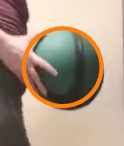
\includegraphics[width=5cm]{img/ball_circled} }}
	\qquad
	\subfloat[\centering Kamuolys nerastas, kadangi jis deformuotas dėl judėjimo]{{
\includegraphics[width=5cm]{img/ball_notfound} }}
	\caption{Kamuolio kontūrų radimas}
	\label{fig:contours}
\end{figure}

Dėl šių trūkumų tolimesniam vaizdo atpažinimui nuspręsta taikyti kamuolio atpažimo pagal spalvą metodus.

\subsection{Nagrinėtų atpažinimo metodų palyginimas}

Tam, kad būtų palygintas šių metodų spartumas bei tikslumas tarpusavy, nuspręsta juos panaudoti sprendžiant praktinę problemą: vaizdo įraše suskaičiuoti, kiek žmogus atliko žingsnių. Žingsnių skaičiavimo algoritmas - gana paprastas, nereikalaujantis daug papildomų sudėtingų skaičiavimų, tad jis puikiai tinka įvertinti pačio vaizdo atpažinimo metodo tinkamumą.  

Žingsnių skaičiavimo algoritmas yra žingsnių taisyklės pažeidimo atpažinimo dalis, plačiau apibūdintas 4 skyriuje. Žmogaus skeleto (pozos) bei spalvinio atpažinimo metodai įgyvendinti tuo pačiu algoritmu, kurio metu pėdų (batų) regionai yra išskiriami, ir laikoma, jog žingsnis yra atliktas tada, kai išskirti regionai persikloja - tai reiškia, jog žiūrint iš šono, įprasto vaikščiojimo metu viena koja trumpai pridengė kitą. Neuroninių tinklų atpažinimo metu prie atpažintų kojų priskiriamos spalvos, tolimesnis atpažinimas panašus į spalvinį.

Metodo, besiremiančio skirtumais tarp kadrų, žingsnių atpažinimo procesas aprašytas 3.2.2 poskyryje.

Visuose vaizdo įrašuose žmogus dėvi raudonus batus, tam, kad veiktų spalvomis paremti atpažinimo metodai ir juos būtų galima lyginti su kitais. Vaizdo įrašų sukurta septyni, juose - skirtingas apšvietimas, nuotolis iki žmogaus, žingsniai atliekami skirtingu tempu ir kamera filmuoja skirtingais kampais. 

Algoritmai buvo patikrinti kelis kartus su tais pačiais įrašais, siekiant sumažinti įvairių kitų kompiuteryje vykstančių procesų įtaką vaizdo apdorojimo greičiui. 


\begin{table}[H]\footnotesize
	\centering
	\caption{Vaizdo įrašai ir jų aprašymai}
	{\begin{tabular}{|p{2cm}|p{8cm}|p{2cm}|} \hline
			\textbf{Vaizdo įrašo nr.} & \textbf{Aprašymas}  & \textbf{Trukmė (s)} \\
			\hline
			1  & Besikeičiantis apšvietimas, žaidėjas eina įstrižai nuo kameros, vaizdo įrašas filmuotas vertikaliai & 12      \\
			\hline
			2  & Žaidėjas eina atgal, kamera filmuoja iš priekio, filmuota horizontaliai          & 2 \\
			\hline
			3  & Žaidėjas vaikšto gan tolokai nuo kameros, filmuota horizontaliai       	 & 5 \\ 
			\hline
			4  & Žaidėjas labai arti kameros, filmuota horizontaliai       
		 	& 7  \\ \hline
			5  & Žaidėjas vaikšto gan tolokai nuo kameros, filmuota vertikaliai, žaidėjas matomas pilnai    & 8    \\
			\hline
			6  & Prastas apšvietimas, žaidėjas gan arti kameros, filmuota horizontaliai       
			& 8 \\
			\hline
			7  & Žaidėjas toli nuo kameros, atsiranda antras žaidėjas, filmuota horizontaliai. Tikimasi, kad bus suskaičiuota abiejų žaidėjų žingsnių suma   & 10     \\
			\hline
	\end{tabular}}
	\label{tab:openposevslightweight}
\end{table}


\begin{table}[H]\footnotesize
	\centering
	\caption{Spalvinio vaizdo atpažinimo žingsnių skaičiavimo eksperimento rezultatai}
	{\begin{tabular}{|p{3cm}|p{3cm}|p{3cm}|p{3cm}|} \hline
			\textbf{Vaizdo įrašo nr.} & \textbf{Atlikta žingsnių} & \textbf{Algoritmo suskaičiuota žingsnių} & \textbf{Vidutinė vaizdo apdorojimo trukmė (ms)} \\
			\hline
			1  & 10    & 13    & 6035    \\
			\hline
			2  & 3    & 0  & 4681     \\
			\hline
			3  & 4    & 2   & 12600    \\
			\hline
			4  & 7    & 7  & 4126     \\
			\hline
			5  & 5    & 5  & 4029     \\
			\hline
			6  & 7    & 6  & 3949     \\
			\hline
			7  & 10    & 6  & 4235     \\
			\hline
	\end{tabular}}
	\label{tab:colorresults}
\end{table}

\begin{table}[H]\footnotesize
	\centering
	\caption{Vaizdo atpažinimo pagal skirtumus žingsnių skaičiavimo eksperimento rezultatai}
	{\begin{tabular}{|p{3cm}|p{3cm}|p{3cm}|p{3cm}|} \hline
			\textbf{Vaizdo įrašo nr.} & \textbf{Atlikta žingsnių} & \textbf{Algoritmo suskaičiuota žingsnių} & \textbf{Vidutinė vaizdo apdorojimo trukmė (ms)} \\
			\hline
			1  & 10    & 9    & 4807    \\
			\hline
			2  & 3    & 4  & 5488     \\
			\hline
			3  & 4    & 4   & 11529    \\
			\hline
			4  & 7    & 10  & 2164     \\
			\hline
			5  & 5    & 2  & 3147     \\
			\hline
			6  & 7    & 8  & 3012     \\
			\hline
			7  & 6    & 4  & 3983     \\
			\hline
	\end{tabular}}
	\label{tab:diffresults}
\end{table}

\begin{table}[H]\footnotesize
	\centering
	\caption{Vaizdo atpažinimo su neuroniniais tinklais žingsnių skaičiavimo eksperimento rezultatai}
	{\begin{tabular}{|p{3cm}|p{3cm}|p{3cm}|p{3cm}|} \hline
			\textbf{Vaizdo įrašo nr.} & \textbf{Atlikta žingsnių} & \textbf{Algoritmo suskaičiuota žingsnių} & \textbf{Vidutinė vaizdo apdorojimo trukmė (ms)} \\
			\hline
			1  & 10    & 8    & 12859    \\
			\hline
			2  & 3    & 0  & 7196     \\
			\hline
			3  & 4    & 4   & 14565    \\
			\hline
			4  & 7    & 0  & 1257     \\
			\hline
			5  & 5    & 5  & 11638     \\
			\hline
			6  & 7    & 8  & 12438     \\
			\hline
			7  & 6    & 6  & 10045     \\
			\hline
	\end{tabular}}
	\label{tab:poseresults}
\end{table}

Palyginę rezultatus matome, jog neuroniniais tinklais paremtas atpažinimas yra tiksliausias, nors ir apdoroti vaizdo įrašą užtrunka daugiausiai laiko. Atpažinimas remiantis skirtumais - greičiausias, tačiau mažiausias yra jo tikslumas, o atpažinimas paremtas spalvomis yra per vidurį. 

Spalvomis paremtas atpažinimas yra mažiausiai tikslus, kai varijuoja apšvietimas arba jis yra prastas, taip pat - jei kadre yra kitų objektų ar žaidėjų, kurių spalvos sutampa su dominančiomis spalvomis. Taip pat šiuo atpažinimu paremtas algoritmas vienintelis, galintis apskaičiuoti žaidėjo atliktus žingsnius iš priekio. 

Iš rezultatų apdorojant vaizdo įrašą nr. 4 galime pastebėti, jog neuroniniais tinklais paremtas atpažinimo metodas neatpažįsta žingsnių, kai žaidėjas yra per arti kameros ir nebesimato jo pilnos figūros, tuo tarpu vaizdo įrašas nr. 7 parodo, jog šis atpažinimo metodas puikiai susidoroja su atvejais, kai yra daugiau žmonių, nei vienas. 

Apibendrinus - spalviniai vaizdo atpažinimo metodai tinka tuomet, kai prie dominančių objektų galime priskirti unikalias spalvas, jos nekinta, neatsiranda naujų, o apšvietimas išlieka puikus - visa tai indikuoja, jog vaizdo įraše fonas ir aplinka turi būti griežtai kontroliuojami ir iš anksto paruošti. Skirtumais paremti atpažinimo metodai labiausiai tinka tais atvejais, kai juos naudojantys algoritmai yra paprasti bei nereikalaujantys didelio tikslumo, siekiant išgauti didžiausią spartumą. Neuroniniais tinklais paremti atpažinimo metodai yra itin tikslūs, tačiau apdorojimo trukmė yra šiek tiek ilgesnė.

\section{Krepšinio taisyklių pažeidimo atpažinimas}

Šiame darbe bus nagrinėjamos kelios taisyklės.

\subsection{Žingsnių taisyklė}
Žingsnių (\textit{angl.} traveling) taisyklė yra aprašyta oficialioje NBA taisyklių knygelės 10 taisyklės 13 skyriuje. Jos formuluotė, kuria remiasi analizė, atlikta šiame darbe, yra tokia: 
\begin{itemize}
	\item Žaidėjas, varydamas kamuolį, gali padaryti du žingsnius prieš sustojant arba kamuolį metant ar atiduodant \cite{nba-rules}. 
\end{itemize}
Būdų pažeisti šią taisyklę yra gausu, tačiau šiame darbe fokusuojamasi į atvejį, kai žaidėjas suėmęs kamuolį atlieka daugiau nei du žingsnius. Tam, kad atlikti žingsniai būtų laikomi kaip pažeidžiantys taisyklę, kamuolys turi būti nemušamas į žemę, o laikomas rankose - krepšinyje tai dažniausiai nutinka prieš metant kamuolį į krepšį, kai yra atliekamas dvižingsnis (NBA tai vadinama kamuolio surinkimu (\textit{angl.} gathering)). Taigi, algoritmas, siekiantis atpažinti šios taisyklės pažeidimą, privalo taip pat gebėti atpažinti, kada kamuolys yra rankose, ir tuomet skaičiuoti atliktų žingsnių skaičių. 
\subsection{Žingsnių taisyklės pažeidimo atpažinimo algoritmas}

Algoritmo reikalavimai: nustatytos rankų, kojų bei kamuolio vietos paveikslėlyje. Apibendrintas algoritmas užsirašytų šitaip: 

\begin{enumerate}
	\item Nuskaitomas kadras.
	\item Nustatoma, ar kamuolys yra laikomas rankose.
	\item Tol, kol kamuolys yra rankose, vykdomas žingsnių skaičiavimo algoritmas.
	\item Jei per intervalą, kai kamuolys yra laikomas rankose, buvo atlikti daugiau nei 2 žingsniai - grąžinamas rezultatas, jog taisyklė pažeista.
\end{enumerate}

  
Algoritmui vienas po kito pateikiami vaizdo įrašo kadrai, kurie yra apdorojami po vieną. Po anksčiau aprašytų atpažinimo metodų turima pakankamai informacijos nustatyti, kur kiekviename kadre yra ranka, kojos ir kamuolys. OpenCV įgalina visų minėtųjų metodų metu išgautą informaciją reprezentuoti loginėse vienetų bei nulių matricose, kur vienetai žymi objekto buvimą tam tikrame plote. 

Tam, kad būtų nustatyta, ar kamuolys yra laikomas rankose, su išskirtomis kamuolio ir rankų užimamą erdvę kadre reprezentuojančiomis loginėmis matricomis atliekama Hadamardo daugyba, t.y. kiekvienam matricos elementui atliekama disjunkcija su toje pačioje vietoje esančiu elementu iš kitos matricos. Rezultate gaunama matrica, žyminti sritį, kur rankos bei kamuolys persikloja. Tai reiškia, jog kamuolio ir rankų pozicija kadre sutampa, tačiau tam tikra rankos dalis yra arčiau kameros ir šiek tiek užstoja kamuolį. 

\begin{figure}[H]
	\centering
	\subfloat[\centering Ranka]{{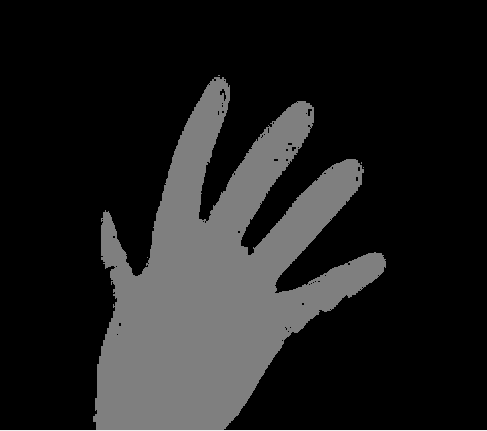
\includegraphics[width=5cm]{img/hand.png} }}
	\qquad
	\subfloat[\centering Kamuolys]{{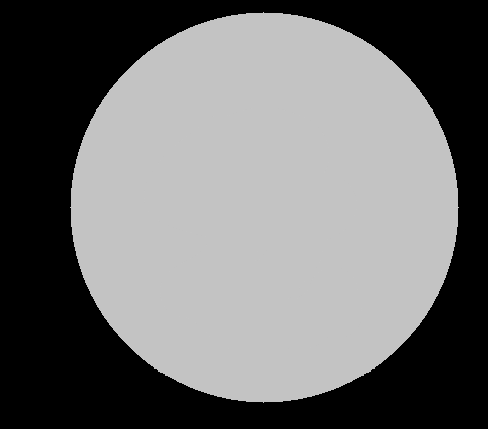
\includegraphics[width=5cm]{img/ball.png} }}
	\qquad
	\subfloat[\centering Ranka arba kamuolys]{{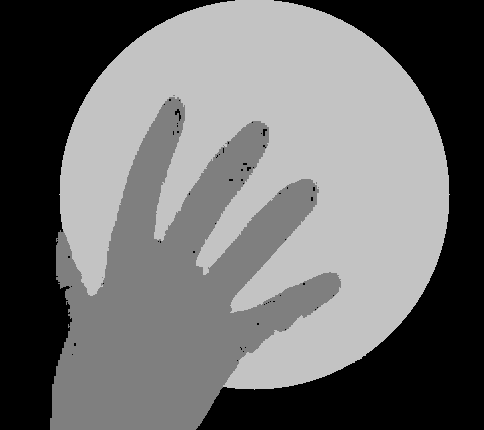
\includegraphics[width=5cm]{img/hand_or_ball.png} }}
	\qquad
	\subfloat[\centering Ranka ir kamuolys (Hadamardo daugyba)]{{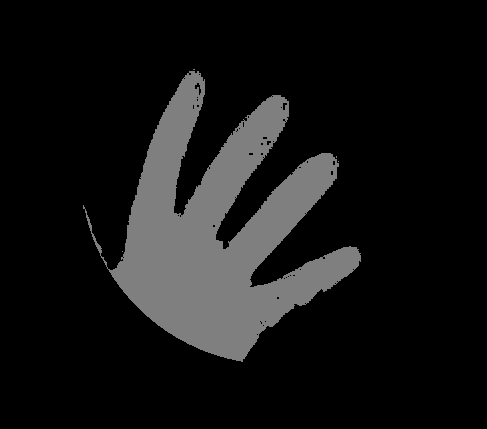
\includegraphics[width=5cm]{img/hand_and_ball.png} }}
	\caption{Kamuolio ir rankų santykio nustatymas}
	\label{fig:hand_and_ball}
\end{figure}

Žingsnių skaičiavimas yra gan kompleksiška problema: ganėtinai sunku apibrėžti universalų būdą atpažinti atliktus žingsnius iš bet kokio kampo. Paprastumo dėlei nuspręsta žingsniųs skaičiuoti tik iš žiūrint šono. Žingsnių skaičiavimo algoritmas remiasi išskirtų kojų regionų kontūrų skaičiavimu. Jei kontūrų suskaičiuota vienas, o prieš tai jų buvo du, galima teigti kad 1) Nerasta informacijos apie vieną iš pėdų (išėjo iš kadro arba nepavyko atpažinimas) arba 2) Žingsnis, žiūrint iš šono, yra toje fazėje, kai viena pėda pridengia (arba yra netoli) kitą. Tam, kad būtų galima atmesti pirmąjį atvejį, laikoma informacija apie atpažintus objektus - jei jų yra vienas, tuomet tai, kad rastas tik vienas kontūras, nekeičia turimų suskaičiuotų žingsnių kiekio. 

Žingsnių skaičiavimo algoritmą, kuris taikytinas reikiamą informaciją išgavus spalviniais atpažinimo metodais arba neuroninių tinklų pagalba, galima apibrėžti taip:

\begin{enumerate}
	\item Išskiriami kojų (batų) regionai.
	\item Suskaičiuojami kontūrai.
	\item Jei kontūrų yra daugiau nei vienas - pasižymima, jog sankirta neįvyko. 
	\item Jei kontūras yra vienas, sankirta dar nebuvo įvykus ir išskirtų regionų skaičius yra daugiau, nei vienas- pasižymima, jog sankirta įvyko ir padidinamas žingsnių skaičius. 
\end{enumerate}

\begin{figure}[H]
	\centering
	\subfloat[\centering Žingsnio pradžia, randami du kontūrai]{{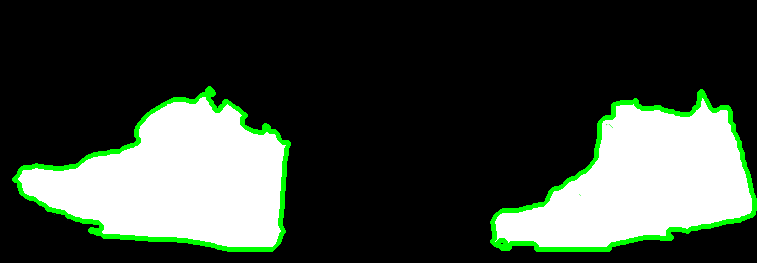
\includegraphics[width=5cm]{img/step_contours1.png} }}
	\qquad
	\subfloat[\centering Žingsnis tęsiasi, kontūrai vis dar du]{{
\includegraphics[width=5cm]{img/step_contours2.png} }}
	\qquad
	\subfloat[\centering Įpusėjęs žingsnis, kontūrai susilieja į vieną]{{
\includegraphics[width=5cm]{img/step_contours3.png} }}
	\caption{Žingsnio atpažinimo procesas skaičiuojant kontūrus}
	\label{fig:hand_and_ball}
\end{figure}

Šis žingsniavimo atpažinimo metodas taikytinas tik tada, kai žingsnis yra kiek galima labiau natūralus, t.y. kojos nėra keliamos per aukštai ir pėdos įpusėjus atliekamam žingsniui yra netoli viena kitos. Lankstesnis yra skirtumais tarp kadrų paremtas algoritmas, atpažįstantis, kada atliktas bet koks judėjimas, tačiau jo tikslumas yra prastas.

Turint informaciją apie kamuolio laikymą tam tikrame laiko intervale ir per jį atliktų žingsnių kiekį, galime daryti išvadą, kad žingsnių taisyklė yra pažeista, kai per minėtą intervalą yra atlikti daugiau nei 2 žingsniai. 

\subsubsection{Būsenos saugojimas}
Atliekant pradinius bandymus su algoritmu pastebėta, jog viena iš problemų, kylančių iš metodų, nustatančių, ar kamuolys yra rankose, tai išskirtų rankų bei kamuolio regionų plotų nepastovumas priklausomai nuo apšvietimo ir kitų faktorių. Tai reiškia, jog laiko intervalas, kada kamuolys yra laikomas rankose, gali būti su trūkiais, indikuojančiais, kad tą laiko momentą nepavyko nustatyti, ar kamuolys yra rankose. Žingsnių skaičiavimo algoritmas skaičiuoja žingsnius tik tada, kai kamuolys yra rankose, tad intervalui nutrūkus dėl netikslaus atpažinimo, skaičiavimas prasidės iš naujo. 

Informacija apie kamuolio buvimą rankose yra renkama ne iš vieno kadro, o iš kelių, ir darant prielaidą, jog rankose esančio kamuolio judėjimo greitis yra arti nulio, galima teigti, jog tokia būsena turėtų nepasikeisti tam tikrą skaičių kadrų. Kitaip tariant, su kiekvienu kadru išsaugoma būsena, ar kamuolys yra rankose ar ne:

\begin{figure}[H]
	\centering
	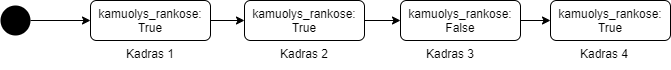
\includegraphics[scale=0.6]{img/state}
	\caption{Būsenos saugojimo pavyzdys kiekviename kadre}
	\label{img:state}
\end{figure}

Išsaugojus būseną suskaičiuojama, kokia buvo jos vidutinė reikšmė per pastaruosius n kadrų: 

\begin{equation}\label{eq:avg_state}
	M_{\textit{vid. būsena}} = \sum_{n=i-x}^{i} \frac{S(n)}{n},
\end{equation}

kur \textit{i} žymi einamo kadro numerį, \textit{x} - konstantą, nurodančią dominančių kadrų skaičių, \textit{S} - \textit{n}-tojo kadro būseną, kur 1 indikuoja kamuolio buvimą rankose, o 0 - atvirkščiai.

Jei vidutinė būsena yra didesnė už tam tikrą iš anksto nustatytą konstantą, pvz., 0.3, galima teigti, jog kamuolys vis dar yra rankose - tam, kad ši reikšmė pasikeistų, turi praeiti bent keli kadrai, pakeičiantys būsenos vidurkį. 

Šis būsenos skaičiavimo būdas atliekant pradinius bandymus su programinės įrangos kodu pasirodė gana naudingas siekiant sumažinti įvarius būsenų svyravymus, kylančius iš atpažinimo netikslumo, tad jis taip pat yra įgyvendintas ir kitame taisyklės pažeidimo algoritme. 

\subsection{Dvigubo varymo taisyklė}
Pagal NBA taisyklių knygelės 10 taisyklės 2 skyriaus c dalį, žaidėjas negali tęsti kamuolio varymo jei jį pats sustabdė. Scenarijai, kada varymas laikomas sustabdytu, aprašyti 4 taisyklės 2 skyriuje. Varymas sustoja, kai kamuolys yra suimamas abejomis rankomis, atiduodamas kitam žaidėjui, metamas į krepšį ar prarandamas kuriuo nors kitu būdu. 

Žaidėjas varymą gali tęsti jei kamuolį atidavus komandos draugui jis buvo grąžintas atgal, taip pat jei po metimo į krepšį žaidėjas pats kamuolį atsikovoja. Visus taisyklei aktualius varymo scenarijus galima supaprastinti į vieną: kamuolys yra suimamas abejomis rankomis. Tam įvykus, žaidėjas gali tik atiduoti kamuolį, mesti į krepšį arba laukti, kol pasibaigs atakai skirtas laikas. 

Taisyklės pažeidimo atpažinimo algoritmas turi atpažinti, jog varymas yra sustojęs, taip pat nustatyti, kada kamuolys buvo išmestas iš rankų ir vėl pagautas (pvz. atliekant varymą antrą kartą). Paprastumo dėlei kuriant algoritmą priimta, jog situacija, kai sustabdžius varymą kamuolys yra išmetamas į orą ir vėl pagaunamas yra taisyklės pažeidimas - tokį veiksmą iš algoritminio atpažinimo perspektyvos sunku atskirti nuo pasavimo ar metimo į krepšį dėl tikslesnių apibrėžimų trūkumo bei subjektyvumo vertinant veiksmo intenciją. Panašus scenarijus apibūdinamas NBA taisyklių 13 skyriuje - žaidėjas metęs ar atidavęs kamuolį negali jo paliesti nepažeidęs taisyklės, jei kamuolio prieš tai nepalietė komandos draugas, priešininkas ar kamuolys neatsimušė nuo lentos ar lanko. Taigi, sustabdžius varymą, kamuolio pagavimas jį išmetus aukštyn ar žemyn yra laikytinas kaip pažeidžiantis taisykles. 

\subsection{Dvigubo varymo taisyklės atpažinimo algoritmas}

Šiam algoritmui, kaip ir žingsnių taisyklės atpažinimo algoritmui, būtina sąlyga - informacija apie kojų (pėdų), kamuolio ir rankų padėtį kadre. Supaprastinta algoritmo versija atrodo taip: 

\begin{enumerate}
 	\item Nuskaitomas kadras.
 	\item Nustatoma, ar varymas yra sustabdytas.
 	\item Nustatoma, ar kamuolys yra išmetamas iš rankų.
 	\item Jei kamuolys yra žaidėjo vėl pagaunamas, grąžinama, kad taisyklė yra pažeista.
\end{enumerate}

Varymo sustabdymą indikuoja tai, jog po varymo kamuolys buvo suimtas abejomis rankomis. Tai atpažinti, jei žaidėjas yra filmuojamas iš priekio, galima atlikus Hadamardo daugybą su išskirtomis rankų ir kamuolio sritį reprezentuojančiomis matricomis (darant prielaidą, jog jų dimensijos sutampa):

\begin{equation}\label{eq:double_dribble}
	M_{kamuolys\ rankose} = M_{kamuolys} \odot (M_{\textit{kairė\ ranka}} + M_{\textit{dešinė\ ranka}}).
\end{equation}

\ref{eq:double_dribble} lygtyje M reiškia loginę matricą, reprezentuojančią tam tikros kūno dalies sritį kadre. 

Šis būdas netinkamas tada, kai žaidėjas yra filmuojamas iš šono - tuomet spalviniais bei žmogaus pozos atpažinimo metodais neįmanoma nustatyti, kur yra žaidėjo užstojama ranka, nes jos tiesiog nesimato. Tam, kad dalinai išspręsti šią problemą, galima pasinaudoti įžvalga, jog sustabdžius varymą ir kamuolį suėmus abejomis rankomis, kamuolys bent tam tikrą laiko tarpą lieka rankose. Šis laiko tarpas yra pakankamai reikšmingas, kad būtų galima jį atpažinti apdorojant kadrus vienas po kito. 

Laiko tarpui, kai kamuolys laikomas rankose, nustatymui galima pasinaudoti 4.2.1. poskyriuje aprašytu būsenos saugojimo algoritmu. 

\sectionnonum{Rezultatai ir išvados}
Rezultatų ir išvadų dalyje išdėstomi pagrindiniai darbo rezultatai (kažkas
išanalizuota, kažkas sukurta, kažkas įdiegta), toliau pateikiamos išvados
(daromi nagrinėtų problemų sprendimo metodų palyginimai, siūlomos
rekomendacijos, akcentuojamos naujovės). Rezultatai ir išvados pateikiami
sunumeruotų (gali būti hierarchiniai) sąrašų pavidalu. Darbo rezultatai turi
atitikti darbo tikslą.

\printbibliography[heading=bibintoc]  % Šaltinių sąraše nurodoma panaudota
% literatūra, kitokie šaltiniai. Abėcėlės tvarka išdėstomi darbe panaudotų
% (cituotų, perfrazuotų ar bent paminėtų) mokslo leidinių, kitokių publikacijų
% bibliografiniai aprašai. Šaltinių sąrašas spausdinamas iš naujo puslapio.
% Aprašai pateikiami netransliteruoti. Šaltinių sąraše negali būti tokių
% šaltinių, kurie nebuvo paminėti tekste. Šaltinių sąraše rekomenduojame
% necituoti savo kursinio darbo, nes tai nėra oficialus literatūros šaltinis.
% Jei tokių nuorodų reikia, pateikti jas tekste.

% \sectionnonum{Sąvokų apibrėžimai}
\sectionnonum{Santrumpos}
Sąvokų apibrėžimai ir santrumpų sąrašas sudaromas tada, kai darbo tekste
vartojami specialūs paaiškinimo reikalaujantys terminai ir rečiau sutinkamos
santrumpos.

\appendix  % Priedai
% Prieduose gali būti pateikiama pagalbinė, ypač darbo autoriaus savarankiškai
% parengta, medžiaga. Savarankiški priedai gali būti pateikiami ir
% kompaktiniame diske. Priedai taip pat numeruojami ir vadinami. Darbo tekstas
% su priedais susiejamas nuorodomis.

\section{Neuroninio tinklo struktūra}
\begin{figure}[H]
    \centering
    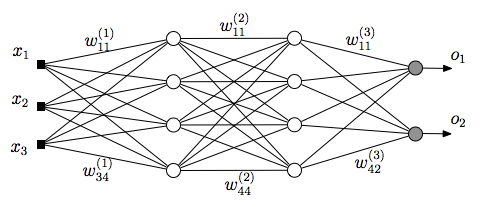
\includegraphics[scale=0.5]{img/MLP}
    \caption{Paveikslėlio pavyzdys}
    \label{img:mlp}
\end{figure}


\section{Eksperimentinio palyginimo rezultatai}
% tablesgenerator.com – converts calculators (e.g. excel) tables to LaTeX
\begin{table}[H]\footnotesize
  \centering
  \caption{Lentelės pavyzdys}
  {\begin{tabular}{|l|c|c|} \hline
    Algoritmas & $\bar{x}$ & $\sigma^{2}$ \\
    \hline
    Algoritmas A  & 1.6335    & 0.5584       \\
    Algoritmas B  & 1.7395    & 0.5647       \\
    \hline
  \end{tabular}}
  \label{tab:table example}
\end{table}

\end{document}
